\newpage
\chapter{REZONANSLAR}\label{ch:Rezonanslar}
Rezonans olayını anlamak için Hamiltonyen'in matris formülasyonu daha uygundur. İki seviyeli bir sistem için gerçel bir Hamiltonyen aşağıdaki gibi yazılabilir.
\begin{equation}
	H = \mqty(0 & H_{12}\\ H_{12} & H_{22} ) \text{ .}
\end{equation}

Rezonans olayını anlayabilmek için sistemi basitleştirelim. Başlangıçtaki durum keti $ \ket{\Psi(R)} = \mqty(1 & 0)^{T} $ olsun, yani başlangıçta sadece elektron nötrinosu olsun. Elektron nötrinosundan x nötrinosuna geçişi $ H_{12} $ elemanı kontrol edecektir. $ H_{12} $ elemanı evrim boyunca sıfır veya sıfıra yakın olduğunda sistem başlangıçtaki özdurumundan sapmayacaktır ve elektron nötrinosu olarak hayatına devam edecektir. Bir diğer taraftan Hamiltonyen'in köşegen terimi $ H_{22} $, $ H_{12} $'ye göre küçük ise sistem başlangıçtaki durumunda olmayacak, iki özdurumun bir süperpoziyonu olacaktır. Herhangi bir $ r $ uzaklığında nötrino çeşni ölçümü yapıldığında x nötrinosu olma olasılığı sıfırdan farklı olacaktır.

Rezonans etkisi, evrimin bir aşamasında $ H_{11}-H_{22} $ farkının sıfır olduğunda ve $ H_{12} $ elemanının sıfırdan farklı olduğu durumda ortaya çıkacaktır. Bu durumda köşegen elemanlar sıfır olacak ve karışım maksimum olacaktır. Bunun anlamı tüm elektron nötrinolarının x nötrinosuna geçmesidir.

Rezonans etkisini genel olarak anlayabilmek için sistemin özdeğerlerine bakmak gerekecektir. Özdeğerlere karşılık gelen özvektörler takip edilerek rezonans durumu incelenebilir. Bunun için özdeğerlerin konuma bağlı değişimi bakılır. Özdeğerler önce birbirlerine yakınlaşır sonra uzaklaşırsa sistem rezonansa girmiş demektir. Bizim ilgilendiğimiz sistemlerde özdeğerler birbirlerine yakınlaşacak ve sistem rezonanslara girecektir.

Rezonans bölgesinde özdurumların birbirlerine \emph{zıplamasının} ifadesini veren Landau - Zener geçiş olasılıklarını hesaplamadan önce Zener'in makalesinde \cite{1932RSPSA.137..696Z} yapılan yaklaşıklıklar açıklanacaktır. 
\begin{enumerate}
	\item Hamiltonyen'in geçişten sorumlu olan elemanı (yukarıdaki basit örnekte $ H_{12} $) konumdan bağımsız olmalıdır.
 	\item Başlangıçtaki anlık (instantaneous) özdurumlar, başlangıç durumu ile aynı olmalıdır. Örneğin başlangıçta sadece elektron nötrinosu var ise sistemin başlangıçtaki özdurumu da çeşni tabanı olmalıdır. Bu yaklaşıklık, Hamiltonyen'deki çeşni geçişinden sorumlu olan elemanının, başlangıçta küçük olmasını zorunlu kılar.
  	\item Özdeğerlerin yakınlaştığı geçiş bölgesinde özdeğer farkları doğrusal olmalıdır.
\end{enumerate}

İki seviyeli sistemlerde LZ geçiş olasılığını bulmak için en genel Hamiltonyen'i yazacağız \cite{1981PhRvA..23.3107R}.
\begin{equation}
	H(r) = \mqty(\omega_{1}(r) & \frac{1}{2} \omega_{0} e^{-i\phi}\\ \frac{1}{2} \omega_{0} e^{i\phi} & \omega_{2}(r) ) \text{ .}
\end{equation}
Burada $ \omega_{0} $, birinci yaklaşıklıktan dolayı konumla değişmemektedir. Bizim kullanacağımız Hamiltonyenler gerçel olduğu için sanal $ \phi $ fazını sıfır alacağız. Bunlara ek olarak çoğunlukla izsiz Hamiltonyenler ile çalışacağımız için $ \omega_{1}+\omega_{2} $ terimi de sıfır olacaktır. 

Bu Hamiltonyen'in özdeğerleri, 
\begin{equation}
	\omega_{a,b} = \frac{1}{2} \pm \sqrt{\qty(\omega_{1}(r)-\omega_{2}(r))^{2}+ \omega_{0}^{2}} \text{ ,}
\end{equation}
şeklinde yazılır. Eğer Hamiltonyen'in köşegen olmayan terimi sıfır olursa, özdeğerler çakışabilir. Böyle bir durumda, özdeğerlerin çakıştığı noktanın özel bir anlamı yoktur. Eğer köşegen olmayan terim sıfır olmaz ise özdeğerler, çakışma noktası etrafında birbirlerinden uzaklaşacaktır.

Kaçınan kesişme (avoided crossing), özdeğerlerin birbirlerine yaklaşması ve ardından ayrılması olarak karakterize edilir. Özdeğerlerin yakınlaşması \ref{fig:avoidCrossing} numaralı şekilde gösterilmiştir. Bu şekilde birbirlerine en yakın olunan nokta $ q_{c} $ noktasıdır. $ q $, Hamiltonyen'i parametrize eden değişkendir. Bizim ilgileneceğimiz sistemler konuma göre evrilecektir. Bundan dolayı kritik nokta $ q_{c} $, kritik uzaklık $ r_{c} $ olacaktır. Kritik noktanın diğer noktalardan ayrılan özelliği, evrim boyunca özdeğerlerin birbirine en yakın olduğu nokta olmasıdır. İşte bu noktada da rezonans meydana gelmektedir. $ \omega_{a}-\omega_{b} $ ise geçişin genişliğini, $ \omega_{0} $ ise özdeğerlerin ne oranda açıldığını karakterize eder. Eğer $ \omega_{0}/\dv{(\omega_{a}-\omega_{b})}{r} $ küçük ise durumlar arası geçiş diyabatiktir, tersi ise adyabatiktir.
\begin{figure}[hbt!]
	\centering
	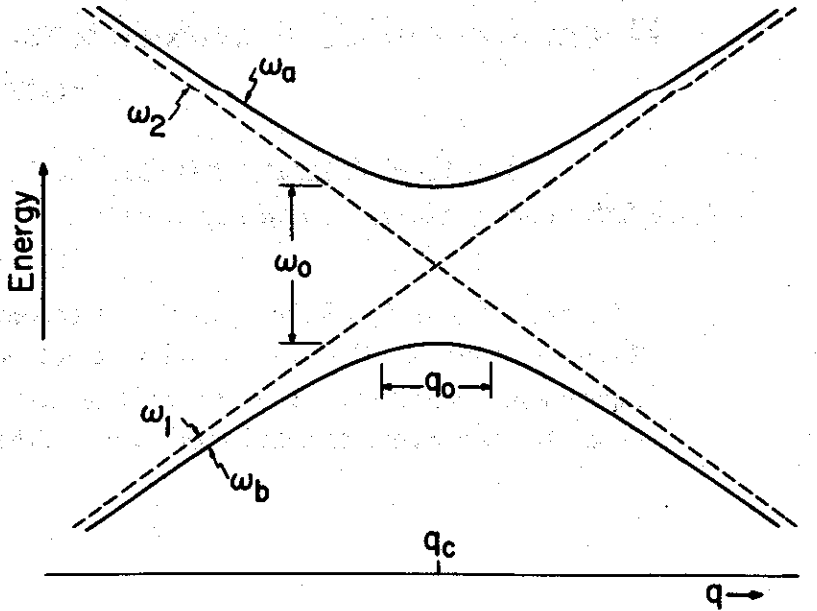
\includegraphics[width=0.5\textwidth]{figures/Avoid_Crossing_With_Paramters.png}
	\caption[Özdeğerlerin Kaçınan Kesişmeleri]{Özdeğerlerin Kaçınan Kesişmeleri. Bu grafik \cite{1981PhRvA..23.3107R} numaralı kaynaktan alınmıştır.}
	\label{fig:avoidCrossing}
\end{figure}

Geçiş olasılığını verecek olan $ \Gamma $ parametresi yani \emph{adyabatisite parametresi} aşağıdaki gibi tanımlanır.
\begin{equation} \label{eqn:LZ_Gamma_def}
	\Gamma = \eval{\frac{\omega^{2}_{0}}{4 \dv{r} \qty[\omega_{1}(r)-\omega_{2}(r)]}}_{r=r_{c}} \text{ .}
\end{equation}
Burada $ \Gamma $ parametresi hesaplanırken, türev alındıktan sonra uzaklık yerine rezonansın uzaklığı yani kritik uzaklık $ r_{c} $ konulmalıdır. Geçiş olasılığını elde etmek için $ r_{\text{başlangıç}} \rightarrow -\infty $ ve $ r_{\text{bitiş}} \rightarrow \infty $ limiti alınırsa sonuç 
\begin{equation}\label{eqn:LZOlasilik}
	P = e^{-2\pi \Gamma}
\end{equation}
şeklinde olur. Bu sonuç Landau \cite{1571980074879151104} ve Zener \cite{1932RSPSA.137..696Z} tarafından birbirlerinden bağımsız olarak elde edilmiştir. Burada başlangıç ve bitiş noktalarının sonsuzda alındığını vurgulamak gerekir, çünkü rezonans noktasının simülasyonun sınır noktalarında olmaması gerekir. Rezonans noktaları sınır noktalarına yakınlaştıkça \eqref{eqn:LZOlasilik} numaralı formül geçersiz olmaya başlayacaktır. Bu sınırlama yukarıda bahsedilen ikinci yaklaşıklık ile uyumludur, çünkü rezonans noktası başlangıç noktasına yakın olduğunda sistemin başlangıç durumu özdurumda olmayacaktır.

Rezonans noktasını belirlemek için Hamiltonyen'i köşegenleştiren dönüşüm matrisi incelenir. Dönüşüm matrisinin efektif açı bağımlılığı \eqref{eqn:appBloch_B_Ozvec} numaralı özvektörlerden gözükmektedir. Efektif açıyı betimleyen tanjant formülüne bakılarak bu nokta belirlenir.
\begin{equation}
	\tan 2\alpha = \frac{2\mel{\nu_{e}}{\hat{H}}{\nu_{x}}}{\mel{\nu_{e}}{\hat{H}}{\nu_{e}} - \mel{\nu_{x}}{\hat{H}}{\nu_{x}}} \text{ .}
\end{equation}
Burada payda sıfır olduğunda sistem rezonansa girecektir. Yani $ \eval{\qty({\omega_{1}(r)-\omega_{2}(r)})}_{r=r_{c}} =0 $ olmalıdır. Not edilmelidir ki, köşegen olmayan terim $ \mel{\nu_{e}}{\hat{H}}{\nu_{x}} $ terimi sıfır veya çok çok küçük olursa rezonans meydana gelmez. Paydanın sıfır olması demek, iki durum arasında karışımın maksimum olması demektir. Yani iki çeşni arasındaki geçiş maksimum değere $ r_{c} $'de ulaşır.

Eğer birden fazla rezonans meydana gelirse geçiş genlikleri çarpılır.
\begin{equation}\label{eqn:LZamplitude}
	A(r) = A_{1}(r_{c_{1}}) \times A_{2}(r_{c_{2}})
\end{equation}
Bu formülün kullanılabilmesi için iki farklı rezonansın birbirinden yeteri kadar ayrılmış olması gerekmektedir. Yani birinci rezonans tamamlandıktan sonra ikinci rezonansın başlaması gerekir. Aksi taktirde rezonanslar arasında karışma (interference) meydana gelir. Karışma meydana geldiğinde $ P_{LZ} $ formülü çalışmaz. İki rezonansın birbirine yakınlaşması durumu \ref{sec:OyuncakModel} numaralı bölümde incelenmiştir.

Birden fazla rezonans meydana gelirken her rezonansta aynı özdurumlar arasında geçiş olmayabilir. Bu durumda geçiş genliği matris olarak yazılmalıdır. Bu matrisi oluşturan elemanlar sanal sayı olacaktır ve köşegen elemanlarının mutlak değer karesi ise geçiş olasılığını, $ P_{LZ} $, verecektir.  LZ formülü içerisinde geometrik fazlar (Stokes fazı) ihmal edilmiştir. Yani geçiş matrisi $ A(r) $ saf gerçeldir. \ref{sec:evrim} numaralı bölümde geçiş genliğinin sanal olmasından kaynaklanan ve evrime gelen katkılar hakkında bilgi mevcuttur.

\section{MSW REZONANSI}\label{sec:mswRezonansi}
\paragraph{}
İki çeşnili nötrinolar, boşlukta belli bir açı ile salınır ve bu açı madde içerisinden geçerken \eqref{eqn:MaddeEtk_EffMixAngCosSin} numaralı denklemde tanımlanan efektif bir değere gider. Efektif açı kullanılarak elde edilen köşegenleştirme işleminde özdeğerler elde edilir. Sadece madde etkileşimi ve nötrino salınım Hamiltonyen'i dikkate alındığında hareket denklemi aşağıdaki gibi olur. 
\begin{align}
	i \dv{r} \mqty(\ket{\nu^{M}_{1}}\\ \ket{\nu^{M}_{2}}) =& \mqty(\omega_{1} & -i \dv{r}\theta_{M} \\ i \dv{r}\theta_{M} & \omega_{2}) \mqty(\ket{\nu^{M}_{1}}\\ \ket{\nu^{M}_{2}}) \text{ ,}\\
	i \dv{r} \mqty(\ket{\nu^{M}_{3}}\\ \ket{\nu^{M}_{4}}) =& \mqty(\omega_{3} & -i \dv{r}\overline{\theta}_{M} \\ i \dv{r}\overline{\theta}_{M} & \omega_{4}) \mqty(\ket{\nu^{M}_{3}}\\ \ket{\nu^{M}_{4}}) \text{ .}
\end{align}
Burada hareket denklemini nötrinolar ve antinötrinolar için ayırdık ve \eqref{eqn:NuKim_EoM_Psi} numaralı denklemi soldan $ U^{\dagger}_{M} $ ve sağdan $ U_{M} $ ile çarparak madde tabanına çevirdik. Hareket denklemini madde tabanına yazarken, $ U_{M}\dv{r}U^{\dagger}_{M} $ teriminden efektif açının türevi gelmektedir. Efektif karışım açılarının tanımları \eqref{eqn:MaddeEtk_EffMixAngCosSin} numaralı denklemde verilmiştir. Eğer baryon yoğunluğu ve elektron kesri sabit ise sistem tam adyabatik durumdadır. Yani efektif karışım açısı konuma bağlı olmadığı için madde özdurumlarının birbirine geçişi mümkün değildir. 

Rezonans durumunu incelemek için \eqref{eqn:MaddeEtk_EffMixAngCosSin} numaralıifadelerini tekrar yazalım.
\begin{align}
	\tan 2\theta_{M} =& \frac{\tan 2\theta}{1- \frac{V_{CC}}{2\Delta c_{2\theta}}} \text{ ,} \\
	\tan 2\overline{\theta}_{M} =& \frac{\tan 2\theta}{1+ \frac{V_{CC}}{2\Delta c_{2\theta}}} \text{ ,}
\end{align}
Yukarıdaki ifadede tanjant ifadesini sonsuza götüren yani paydayı sıfır yapan özel koşula \emph{rezonans koşulu} adı verilir ve aşağıdaki gibi yazılır.
\begin{align}\label{eqn:MSWresonanceConditions}
	V_{CC}(r_{MSW}) + 2\Delta c_{2\theta} =& 0 \text{ ,} \\
	V_{CC}(r_{MSW}) - 2\Delta c_{2\theta} =& 0 \text{ .}
\end{align}
Burada kritik uzaklık yani sistemin MSW rezonansına girdiği uzaklık $ r_{MSW} $ olarak verilmiştir.

Nötrinoların veya antinötrinoların MSW rezonansına girme koşulları sadece yüklü akım etkileşimine bağlıdır. Yüklü akım etkileşiminin de açık ifadesi yazıldığında
\begin{align} 
	\label{eqn:MSWresonanceConditions_explicitNu}\sqrt{2}G_{F}n_{b}(r_{MSW})Y_{e} + 2\Delta c_{2\theta} =& 0 \text{ ,} \\
	\label{eqn:MSWresonanceConditions_explicitNub}\sqrt{2}G_{F}n_{b}(r_{MSW})Y_{e} - 2\Delta c_{2\theta} =& 0 \text{ ,}
\end{align}
elde edilir. Burada elektron kesri, $ Y_{e} $, de konuma bağlı olabilir ancak bu tezde biz konumdan bağımsız alacağız. Bu koşullara bakıldığında nötrinolar ve antinötrinolar aynı anda MSW rezonansına giremezler. Nötrinoların hiyerarşisine göre ya nötrinolar ya da antinötrinolar MSW rezonansına girecektir. Daha açık ifade için \ref{tab:ResonanceCond} numaralı tabloyu inceleyiniz. Ayrıca nötrinoların MSW rezonansından geçmesi için gereken baryon yoğunluğu ve elektron kesri değerleri için \ref{fig:resonance_nb_Ye} numaralı grafiğe bakabilirsiniz.

Yüksek baryon yoğunluğu altında efektif açı küçük bir değer alacaktır. Baryon yoğunluğu azaldığında ve \eqref{eqn:MSWresonanceConditions_explicitNu}, ( \eqref{eqn:MSWresonanceConditions_explicitNub}) numaralı koşul(lar) sağlandığında efektif açı aniden $ \pi/4 $ ye yakınlaşacaktır. Böyle bir durumda $ \ket{\nu^{i}_{M}} $ madde özdurumunun çeşni içeriği değişecektir. Özdeğerlerin konumla değişimi \ref{fig:simpleCaseSemiAdiabFlavContent} numaralı şeklinde verilmiştir. Bu şekilde, özdeğerlerin birbirine yakınlaşıp uzaklaştığı yerde rezonans meydana gelmektedir. Özdeğerlerin üzerinde yazan çeşni vektörleri ise o özdeğere ait özvektördeki en büyük çeşni vektörüdür.

Nötrinolar MSW rezonansından adyabatik veya diyabatik olarak geçebilir. Bu geçişi betimlemek için adyabatisite parametresi yazılabilir \cite{Giunti:2007ry}. 
\begin{align}
	\Gamma_{MSW} = \eval{\frac{\delta \omega_{12}}{\dv{r}\theta_{M}}}_{r_{MSW}} \text{ ,} \\
	\overline{\Gamma}_{MSW} = \eval{\frac{\delta \omega_{34}}{\dv{r}\overline{\theta}_{M}}}_{r_{MSW}} \text{ .}
\end{align}
Bu ifade madde tabanında yazılan Hamiltonyen'in köşegen elemanlarının köşegen olmayan elemanlarına oranıdır. Eğer $ \Gamma_{MSW} $ çok çok büyük ise sistem adyabatiktir. Tam tersi $ \Gamma_{MSW} $ sıfıra yakın ise sistem diyabatiktir. Eğer sistemin özdurumu başlangıçtaki halindeyse evrim adyabatiktir denir.

Adyabatisite parametresi LZ geçiş olasılığından yani \eqref{eqn:LZ_Gamma_def} numaralı denklemden de hesaplanabilir. Her iki ifadeden hesaplanan adyabatisite aynı olacaktır.

\section{SFP REZONANSI}\label{sec:sfpRezonansi}
\paragraph{}
Nötrinolar sadece madde içerisinden geçiyorsa sadece MSW rezonansına girebilir. Nötrino madde etkileşimlerine ek olarak nötrino elektromanyetik etkileşim varlığında ise sistem yeni bir rezonansa yani spin çeşni yalpalama, SFP, (spin flavor precession) rezonansına girebilir. Bu bölümde SFP rezonansı için yapılacak olan tüm prosedür MSW rezonansı ile benzerlik gösterecektir. 

%SFP rezonansı, tarihsel olarak LMA (Large Mixing Angle, $1-4$) rezonansı adı verilmiştir. Nötrino boşluk salınım açısı $ \theta $ üzerindeki büyük belirsizlikten dolayı bu adlandırılma yapılmıştır. Diğeri ise SMA rezonans adlandırması da vardır ve küçük karışım açı anlamına gelen (Small Mixing Angle) $1-2$ rezonansına denk gelmektedir \cite{Friedland:2006xj}.

SFP rezonansından geçen nötrinoların evrimini incelemek için \eqref{eqn:Hamiltonyen_T14} ve \eqref{eqn:Hamiltonyen_T23} numaralı denklemlerde verilen matrislerden hesaplamaya başlanır. İndirgenmiş olan bu Hamiltonyenler'in özdeğerleri hesaplanır. Özdeğerler \eqref{eqn:Ozdeger_EMetkilesim14} ve \eqref{eqn:Ozdeger_EMetkilesim23} numaralı denklemlerde verilmiştir. Ardından efektif elektromanyetik karışım açısı, $ \theta_{EM} $, hesaplanır. Bu açı da \eqref{eqn:theta_EM_hepsi} numaralı denklemde verilmiştir. SFP rezonansına girme koşulu ise, \eqref{eqn:theta_EM_hepsi} numaralı denklemin paydasının sıfır olduğu değerdedir.
\begin{align}\label{eqn:SFPresonanceConditions}
	V_{NC}(r_{SFP}) + V_{CC}(r_{SFP})/2 - 2\Delta c_{2\theta} =& 0 \text{ ,} \\
	V_{NC}(r_{SFP}) + V_{CC}(r_{SFP})/2 + 2\Delta c_{2\theta} =& 0 \text{ .}
\end{align}

MSW rezonansı ile SFP rezonansı arasındaki tek fark, rezonans koşulunda yüksüz akım etkileşim potansiyelinin, $ V_{NC} $, bulunmasıdır. Potansiyellerin açık ifadeleri yazıldığında
\begin{align}
	\label{eqn:SFPresonanceConditions_explicit14}\sqrt{2}G_{F}n_{b}(r_{SFP})(2Y_{e}-1) - 2\Delta c_{2\theta} =& 0 \text{ ,} \\
	\label{eqn:SFPresonanceConditions_explicit23}\sqrt{2}G_{F}n_{b}(r_{SFP})(1-2Y_{e}) - 2\Delta c_{2\theta} =& 0 \text{ ,}
\end{align}
bağıntıları elde edilir. Burada $ r_{SFP} $, rezonansın meydana geldiği uzaklıktır. SFP rezonansının meydana gelmesi için elektron kesri $ Y_{e} $'nin $ 0,5 $ değerinden farklı olması gerekmektedir. Ayrıca elektron kesrinin $ 0,5 $'ten büyük veya küçük olmasına göre $ e-\bar{x} $ veya $ x-\bar{e} $ geçişi belirlenir. Rezonansların oluşma koşulları için \ref{tab:ResonanceCond} numaralı tabloyu bakınız.

Her ne kadar rezonans koşulu içerisinde $ \mu B $ terimi olmasa da, SFP rezonansının meydana gelmesi için elektromanyetik etkileşime ihtiyaç vardır.  $ \mu B $ teriminin büyüklüğü, özdeğerlerin birbirlerine en yakın olduğu noktada, birbirlerinden ne kadar ayrık olduğunu belirleyecektir. Bu da SFP rezonansının adyabatik olup olmadığını belirler. SFP rezonansı için adyabatiklik koşulu aşağıdaki gibi yazılır.
\begin{align}
	\Gamma_{SFP} = \eval{\frac{\mu B}{\dv{r}(\sqrt{2}G_{F}(2Y_{e}-1)n_{b}(r))} }_{r_{SFP}} \text{ ,} \\
	\overline{\Gamma}_{SFP} = \eval{\frac{\mu B}{\dv{r}(\sqrt{2}G_{F}(1-2Y_{e})n_{b}(r))} }_{r_{SFP}} \text{ .}
\end{align}
Yukarıda bağıntı, LZ geçiş olasılığı için elde edilen ifadeden elde edilmiştir. Benzer bir ifade, efektif karışım açısı $ \theta_{EM} $'nin türevi kullanılarak da yazılabilir.
\begin{align}\label{eqn:adyabatisiteSFP}
	\Gamma_{SFP} = \eval{\frac{(\lambda_{1}-\lambda_{2})_{e\bar{x}}}{\dv{r}\theta_{EM}}}_{r_{SFP}} \text{ ,} \\
	\overline{\Gamma}_{SFP} = \eval{\frac{(\lambda_{1}-\lambda_{2})_{x\bar{e}}}{\dv{r}\overline{\theta}_{EM}}}_{r_{SFP}} \text{ .}
\end{align}
Yukarıdaki adyabatisite parametrelerinin arasındaki fark, bu tezde dikkate alınacak dış koşullara göre küçük kalacaktır. Farklar hakkında detaylı bilgi için \cite{Friedland:2005xh} numaralı kaynağa bakınız.

SFP rezonansının adyabatisitesi ile MSW rezonansının adyabatisitesi arasındaki en büyük fark, efektif açılarının uzaklık bağımlılıklarıdır. MSW rezonansındaki uzaklık bağımlılığı sadece baryon yoğunluğundan gelir. SFP rezonansındaki uzaklık bağımlılığında dış manyetik alanın değişimi de önemlidir. Bu da dikkate alındığında $ \theta_{EM} $ açısının konuma göre türevi aşağıdaki gibi olur.  
\begin{equation}
	\dv{r} \barparen{\theta}_{EM} = \frac{\mu}{2 \barparen{M}_{EM}} \qty[\dv{B}{r}\qty(\Delta c_{2\theta}\pm V_{NC} \pm V_{CC}/2) \mp B\qty(\dv{(V_{NC}+ V_{CC}/2)}{r})] \text{ .}
\end{equation}
Dış manyetik alanın konuma bağlılığı \eqref{eqn:adyabatisiteSFP} numaralı denklemin paydasında kendini gösterebileceği gibi payında da gösterecektir. Ancak LZ formülünü kullanabilmemiz için geçişi veren terim, ki burada $ \mu B $, konumdan bağımsız olmak zorundadır. Bundan dolayı dış manyetik alanın rezonans bölgesinde çok değişmediği varsayılacaktır.

Bu kısma kadar yazılan tüm rezonans koşullarını ve adyabatisite parametrelerini elde ederken, potansiyellerin konuma bağlılıklarının rezonans noktasında doğrusal olduğu varsayılmıştır. Bu varsayım adyabatik geçişlerde önemli olmasa da diyabatik geçişlerde önemli hale gelecektir. Maksimal diyabatik MSW rezonans geçişi durumlarında ortalama yaşama olasılığı Parke formülü ile verilir \cite{Parke:1986jy}. Parke formülü de doğrusal potansiyeller için yazılmış olup doğrusal olmayan potansiyelleri için \cite{Kuo:1989qe} numaralı kaynağı ve bu makalenin referanslarına bakınız. MSW rezonansı için yazılan Parke formülü dış manyetik alanın değişimi için yazılamamaktadır. Bu tezde ele alınacak madde ve elektromanyetik potansiyeller konuma doğrusal olarak bağlı değildir ancak rezonans bölgesinde konuma bağlılığın doğrusal olduğu varsayılacaktır. Bir diğer değişle sistemin rezonansa girdiği nokta yakınlarında $ V_{NC}(r)+ V_{CC}(r) $ teriminin doğrusal, $ B(r) $ teriminin ise sabit olduğu varsayılacaktır. Buradan elde ettiğimiz adyabatisite parametreleri ve LZ geçiş olasılığı kullanılacaktır.

Adyabatisite koşullarına bakıldığında hem MSW hem de SFP rezonansı aynı noktada olabilir. Bu noktalar, \ref{fig:resonance_nb_Ye} numaralı şekilde kırmızı ve siyah noktaların üst üste bindiği noktalardır. Bu durumda, SFP rezonansı için elde edilen LZ geçiş olasılığı ve diğer bağıntılar geçersiz olacaktır. Bunun sebebi, SFP rezonans koşulları ve adyabatisite ifadeleri elde edilirken Hamiltonyen $ 2\times2 $ boyuta indirgenmiştir. MSW rezonansı ise Hamiltonyen'in $ 12 $ veya $ 34 $ terimlerinin maksimum olduğunda oluşur. Bundan dolayı MSW ve SFP rezonanslarının meydana geldiği noktalar birbirlerine yakınlaştığında dört çeşni etkileri açığa çıkar ve sayısal çözüme ihtiyaç duyulur.
Bir başka değişle, buradaki formülasyon SFP rezonansı bölgesinde sistemi $ \ket{\nu_{\bar{x}}}-\ket{\nu_{e}} $ alt uzayına indirgeyerek, MSW bölgesinde ise $ \ket{\nu_{\bar{x}}}-\ket{\nu_{\bar{e}}} $ alt uzayına indirgeyerek çalışmaya dayalıdır. Doğal olarak iki rezonans birbirine yakınlaştıkça dinamik $ \ket{\nu_{\bar{x}}}-\ket{\nu_{\bar{e}}}-\ket{\nu_{e}} $ alt uzayına yayılacak ve $ 3\times3 $ bir sistem ele almak gerekecektir.

\begin{table}[hbt!]
	\centering
	\begin{tabular}{c|c|c|c|c|}
	  &
	  & \textbf{IH} & \textbf{NH} & \textbf{Rezonans için} $\mathbf{n_{b}(r)}$ \\ 
	  \hline
	  \multirow{2}{*}{\STAB{\rotatebox[origin=c]{90}{\tiny \textbf{SFP}}}} &     $\nu_{e} \leftrightarrow \nu_{\bar{x}}$ & $ Y_{e}<0.5 $  & $ Y_{e}>0.5 $ & $ 2\Delta\cos 2\theta/ 
     \left(\sqrt{2}G_{F}(2Y_{e}-1) \right)$ \\ \cline{2-5}
     & $\nu_{x} \leftrightarrow \nu_{\bar{e}}$ & $ Y_{e}>0.5 $ & $ Y_{e}<0.5 $ & $ 2\Delta\cos 2\theta/ \left(\sqrt{2}G_{F}(1-2Y_{e})  \right)$ \\ \hline
	  \multirow{2}{*}{\STAB{\rotatebox[origin=c]{90}{\tiny \textbf{MSW}}}} & $\nu_{e} \leftrightarrow \nu_{x}$ & $\times $ & $\checkmark$ & $ 2\Delta\cos 2\theta/ \left(\sqrt{2}G_{F}Y_{e} \right)$\\
	   \cline{2-5}
	   & $\nu_{\bar{x}} \leftrightarrow \nu_{\bar{e}}$
	   &  $\checkmark$ & $\times $ & $-2\Delta\cos 2\theta/ \left(\sqrt{2}G_{F}Y_{e} \right)$\\
	   \hline
	\end{tabular}
	\caption[SFP ve MSW rezonans koşulları]{\label{tab:ResonanceCond}SFP ve MSW rezonans koşulları. Madde arka planı yüksüz olmalı. $ n_{p} = n_{e} $. Son sütun MSW rezonansına girmek için gereken baryon değerini göstermektedir. Üç nötrino çeşnisi için SFP rezonans koşulları için \cite{Akhmedov:2003fu} numaralı kaynağa bakınız.}
\end{table}

\begin{figure}[hbt!]
	\centering
	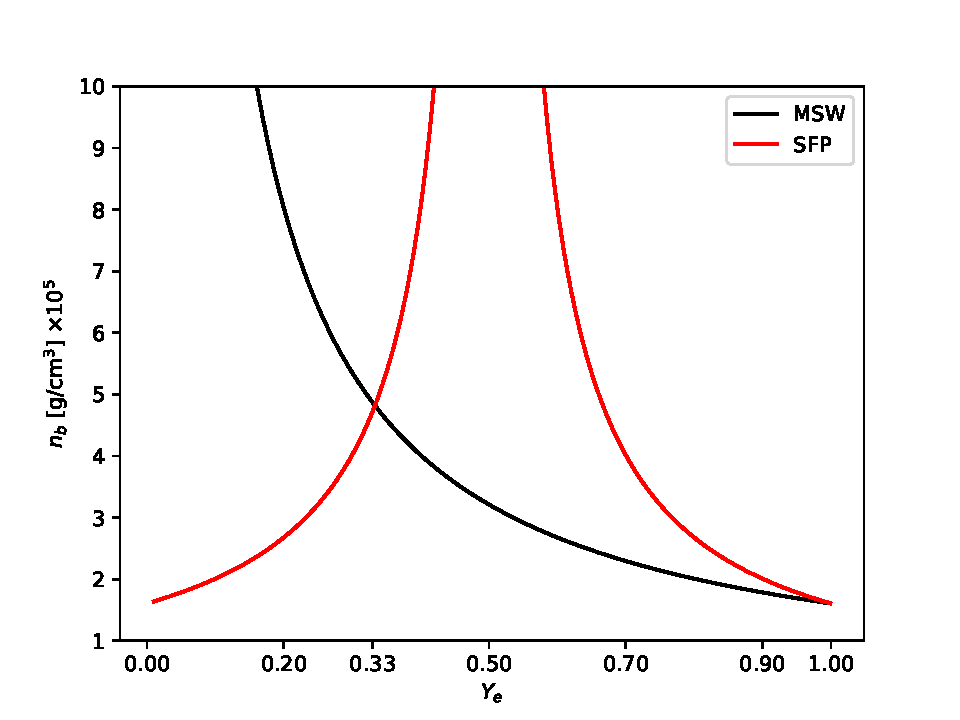
\includegraphics[width=0.8\textwidth]{figures/resonance_nb_Ye.pdf}
	\caption[MSW ve SFP rezonansları]{MSW ve SFP rezonansları. Eğer madde ortamında $ Y_e = 0.33 $, $n_{b}(r) \simeq 5 \times 10^{4} $ g/cm$^{3}$ veya $ Y_e \simeq 1 $, $n_{b}(r) \simeq 2	\times 10^{4} $ g/cm$^{3}$ değerleri mevcut ise MSW ve SFP meydana geldiği uzaklıklar kesişir. Bu şekil $ 1 $ MeV enerjiye ve atmosferik karışım açılarına sahip nötrinolar için hesaplanmıştır. }
	\label{fig:resonance_nb_Ye}
\end{figure}
\begin{figure}[hbt!]
	\centering
	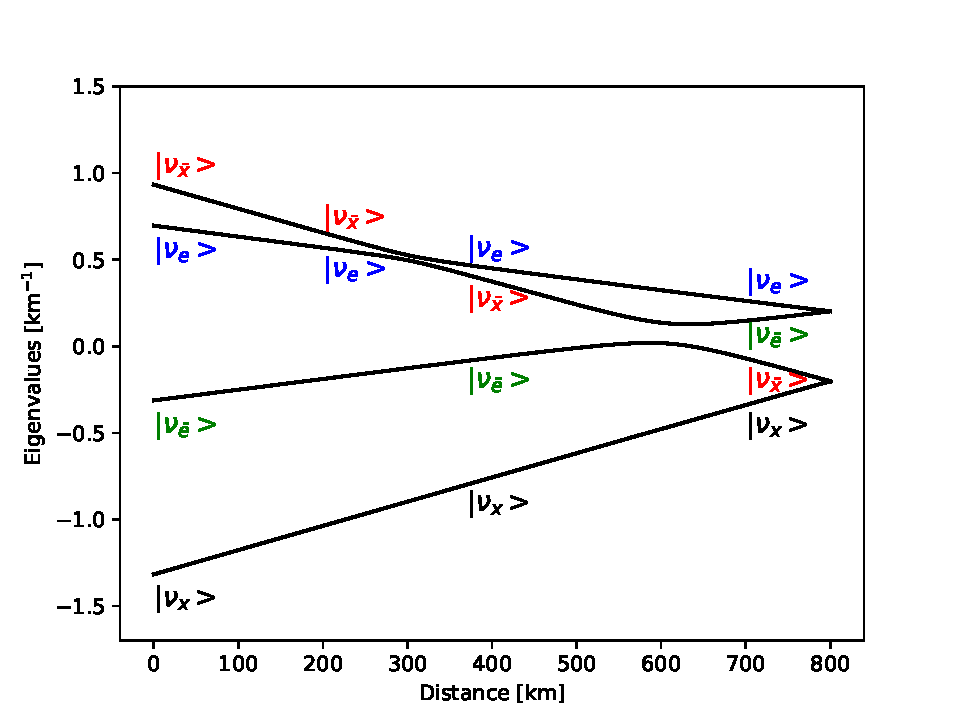
\includegraphics[width=\textwidth]{figures/constant_B_linear_V_flavorContent_16_MeV.pdf}
	\caption[MSW ve SFP Rezonansından geçen nötrinoların çeşni içerikleri]{MSW ve SFP Rezonansından geçen nötrinoların çeşni içerikleri. Bu grafik $ 16 $ MeV için çizilmiştir. Madde profili doğrusal olup manyetik alan ise sabittir.}
	\label{fig:simpleCaseSemiAdiabFlavContent}
  \end{figure}